\section{Datalinklag}
Datalinklaget er laget efter det fysiske. Det yder services til transportlaget og modtager services fra det fysiske lag.
Når datalinklaget tager rollen som afsender, skal det modtage payloads fra transportlaget, samt tage ansvaret for at pakke disse ned i et format, der tillader det modtagende datalinklag at genkende og finde fejl i den transmitterede data.
Når datalinklaget tager rollen som modtager, skal den modtage en bitstrøm fra sit fysiske lag, og er ansvarlig for genkendelse og opdeling af disse i de originale datapakker.
Herefter skal det originale payload fra afsenderens transportlag verificeres og udvindes, således at det kan gives videre til det modtagende transportlag.

\subsection{Afsender}
For at facilitere den logiske forbindelse mellem de afsendende og modtagende datalinklag, er det essentielt at beslutte sig for et pakkeformat, som både afsender og modtager kender til. Der er her fokus på overvejelserne omkring pakkernes størrelse, udformning og afgrænsning, samt hvilken redundant information der tilføjes, for at opnå den førnævnte funktionalitet. Figur \ref{fig:DataLinkLogical} viser datalinklagets placering i den lagdelte programstruktur, samt nogle af de essentielle metoder og den logiske forbindelse mellem to lag der kommunikerer.

\begin{figure}[h!]
\centering
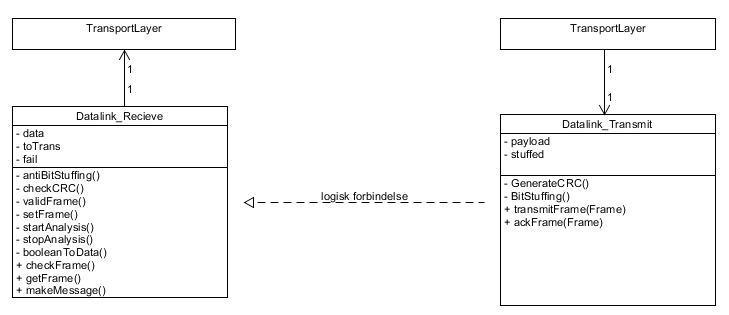
\includegraphics[scale=0.7]{Billeder/DataLinkLogical.PNG}
\caption{Her ses et uddrag fra designklassediagrammet, som viser den logiske forbindelse mellem to datalinklag}
\label{fig:DataLinkLogical}
\end{figure}

\subsubsection{Bit- eller karakter-orienteret protokol}
Datalinklaget skal behandle information som en serie af enten bits eller bytes. Projektets primære mål om at oprette en forbindelse mellem to klienter kan opfyldes med begge protokoltyper, hvor det er relevant at vurdere sekundære ting såsom protokollernes effekt på transmissionshastighed.
I en byte-orienteret protokol behandles data som en streng af karakterer. I denne type kan redundant information kun tilføjes som hele bytes.
En bit-orienteret protokol behandler data som en strøm af bits. Her kan redundant information tilføjes bitvist. 
    Den byte-orienterede protokol virkede i første omgang som det bedste valg, da det primære mål for projektet er at skabe en chat-klient, hvor der udveksles tekst-beskeder, som er lette at pakke ned i en byte-orienteret frame. Samme resultat kan imidlertid også opnås med en bit-orienteret protokol, som i tilgift er mere kompatibel med andre datatyper, og samtidig også mere kompakt når det kommer til tilføjelse af redundant information. Dette giver et kortere pakkeformat og en hurtigere transmission. Det blev også fundet lettere at arbejde med bits, da en CRC-division skulle foretages. Af disse årsager blev en bit-orienteret protokol valgt.

\subsubsection{Fast eller variabel framelængde}
Datalinklagets datapakker kan enten have en fast defineret længde, eller en variabel længde.
Vælges en fast længde på alle pakker, bliver pakkernes længde en afgrænsning i sig selv - og det er således ikke nødvendigt at indsætte start- og stopflag. Hvis en pakke er mindre end den definerede længde, er det nødvendigt at tilføje yderligere, redundante bits for at opfylde pladskravet.
Er pakkernes længde variabel, er det nødvendig at indsætte flag i begyndelsen og slutningen af hver frame. Hvis disse bitmønstre indgår i datastrømmen, er det nødvendigt at indsætte redundante bits i afsenderen, så der ikke findes falske flag, der kan blive misfortolket af det modtagende datalinklag.
Et af projektets primære mål er udviklingen af en chat-klient. Chat-beskeder er af naturlige årsager af meget varierende længde. Af denne årsag er det svært at finde en uniform pakke-længde, der minimerer spild i datatransmissionen. Derfor blev frames med variabel længde valgt.

\subsubsection{Pakkeindhold}
Disse præmisser bliver  bruget til at fastsætte pakkens opbygning og indhold.

\begin{figure}[h!]
\centering
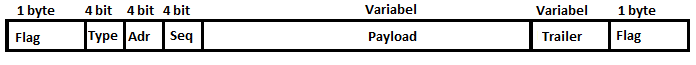
\includegraphics[scale=0.8]{Billeder/DataLinkFrame.PNG}
\caption{Her ses udformningen af en pakke på datalinklagets niveau}
\label{fig:DataLinkFrame}
\end{figure}

\textbf{Flag:} Pakkerne af variabel størrelse markeres gennem hhv. start- og stopflag. Hvis flagene indgår i dataens bitmønster, er det nødvendigt at tilføje bits i datalinklagets afsender, så disse ikke bliver forvekslet med begyndelsen eller afslutningen på en frame. De indsatte bits skal ligeledes fjernes i afsenderen. 

\textbf{Type:} Da transportlaget skal benytte acknowledge-pakker i implementeringen af flow- og fejlkontrol, er det nødvendigt med et type-felt. Dette denoterer pakken som værende enten en kvitterings- eller datapakke. Datalinklaget har fået ansvaret for at tilføje dette felt, da resten af datapakken alligevel opbygges på dette lag, og det derfor er oplagt at tilføje.

\textbf{Adresse:} Ét af projektets sekundære mål, er muligheden for kommunikation mellem mere end to klienter. For at muliggøre dette indsættes et adressefelt, som skal indeholde modtagerens adresse. Dette felt kan desuden benyttes af en afsender, til at sortere egne pakker væk, såfremt disse fejlagtigt skulle blive opfanget.

\textbf{Sekvensnummer:} Med henblik på at holde de enkelte pakker i en begrænset længde, skal længere beskeder opdeles i flere pakker, i hvilken forbindelse det er relevant at operere med et sekvensnummer. Det gør det muligt at detektere dubletter og holde holde styr på rækkefølge.

\textbf{Trailer:} For at hindre korrupt data i at nå de øvre lag, skal der implementeres en form for fejl-kontrol på datalinklaget. Det gøres ved at implementere et CRC, da dette er en del af IP / TCP standarden, som protokollen er inspireret af. Det er samtidig er en simpel og effektiv måde at detektere fejl.
Der er implementeret CRC af varierende størrelser. Dataordet, som består af pakkens header samt payload, får tilføjet nogle redundante bit, og divideres igennem med et generatorpolynomie. Resten fra denne division påsættes til sidst enden af det originale dataord.	Valget af denne CRC-generator påvirker længden af fejl der med garanti bliver fundet, samt sandsynligheden for at detektere burst-fejl med højere længde end generatorpolynomiet.

Når en CRC længde vælges, detekteres alle fejl med en længde lavere eller lig CRC'ets længde. Er fejlens længde 1 længere end CRC'et, udregnes sandsynligheden for detektering af fejl ved følgende ligning:
\begin{equation}
\label{eq:CRCError}
P_{fejl1}=1-(1/2)^{r-1}
\end{equation}

Er fejlen længere end dette, udregnes sandsynligheden for detektion ved:
\begin{equation}
\label{eq:CRCError2}
P_{fejl2}=1-(1/2)^r
\end{equation}
Et CRC8 detekterer alle burst-fejl med en længde under 8. I dette tilfælde kan sandsynligheden for at detektere fejl af højere længde end 10 findes som $1-(1/2)^8 = 99,61\%$
Et CRC16 detekterer alle burst-fejl med en længde under 16. Sandsynligheden for at detektere længere fejl end 18 findes som $1-(1/2)^{16} = 99,9999\%.$
	Det ses, at sandsynligheden for at detektere fejl fra et CRC8 til et CRC16 stiger drastisk. Denne sandsynlighed blev vurderet som værende tilstrækkelig stor, og et CRC16 blev valgt.
    Der blev valgt ikke at fokusere på manuel dimensionering af en generator. Istedet benyttedes et, der med garanti opfylder kravene for gode polynomier\footnote{Data Communications and Networking, kapitel 10.3.4}.


\subsubsection{C++ implementering}
Pakkernes indhold og udformning er implementeret i C++-klassen "Datalink-transmit"


\paragraph{Beholder-format}\hfill \break
I C++ implementeringen af afsenderen, var det oplagt at arbejde med et beholder-format, med beholdere til at indeholde pakkernes forskellige data-elementer.
I denne forbindelse blev der overvejet hhv. arrays og vector-biblioteket i C++. 
Arrays er som udgangspunkt statisk allokerede beholdere.
Vectorer er dynamisk allokerede, og har indbygget funktionalitet til bla. automatisk ændring af størrelse, samt måling af længde. “Bag facaden”, er dette implementeret igennem allokering af mere end den nødvendige hukommelse, og kopiering af vector-indholdet til nye placeringer, når den tilsidesatte hukommelse ikke længere er tilstrækkelig. 
Valget faldt i sidste ende på vectors. De indbyggede funktionaliteter i vector-biblioteket er nyttige, da det ikke på forhånd er nødvendigt at deklarere længden på beholderen, og disse bit-for-bit kan opbygges eller modificeres. Dette er idéelt når der vælges en protokol med variable størrelser på pakker. Såfremt der var blevet valgt en fast størrelse på pakkerne, kunne arrays benyttes istedet, hvilket sparer nogle system-operationer.

\paragraph{Vigtigste metoder}\hfill \break
Afsenderen arbejder med følgende metoder, der implementerer de tidligere nævnte funktionaliteter og principper.
\begin{itemize}[noitemsep]
  \item generateCRC()
  \item bitStuffing()
  \item transmitFrame()
  \end{itemize}
generateCRC og bitStuffing er hjælpemetoder der tilføjer hhv. CRC og bitStuffing til en vector.
transmitFrame opbygger en pakke bit-for-bit i en vector, og sender denne vector videre til sit fysiske lag.

\subsection{Modtager}
Datalinklaget på modtagersiden skal kommunikere logisk med afsenderen, men har adskillige ekstra ansvarsområder. Dette skyldes ét af projektets primære mål om, at korrupt data ikke må nå de højere lag. Afsenderens datalinklag er baseret på en antagelse om, at transportlaget ikke videresender forkert data, men denne garanti eksisterer ikke i modtagerens fysiske lag. Det er derfor ikke tilstrækkeligt kun at aflæse den transmitterede data, den skal også valideres ift. adresse, type og korrekthed.

\subsubsection{Genkendelse og validering}
Modtagerens første opgave er genkendelse af data fra det fysiske lag. Fra udviklingen af det sendende datalinklag vides det, at den relevante information er pakket ind med hhv. start- og stopflag. Modtageren gennemsøger løbende sit fysiske lags buffer for disse flag, mens det også har ansvaret for at tømme denne buffer. Når et flag detekteres i bitmønsteret, indsættes den efterfølgende data i en vector. Denne proces afsluttes når det næste flag findes i det fysiske lags buffer.
    Når relevant data er blevet fundet, skal bitstuffingen fjernes. Herefter skal pakken valideres, hvilket gøres i traileren, der fra afsenderen indeholder et CRC. Modtagerens CRC-dekoder skal foretage samme division som afsenderens, blot med traileren påsat. Er resultatet af denne division 0, accepteres dataen som fejlfri.
    
\subsubsection{Buffering}
Når dataen er valideret, skal den udvindes fra vectoren og gemmes. Til dette benyttes en struct, hvor hhv. adresse, type, sekvensnummer og payload placeres. Denne struct skal placeres i en buffer, hvor den kan tilgås af det modtagende transportlag.

\subsubsection{C++ implementering}
Efter fastsættelsen af modtagerens ansvarsområde og fremgangsmåde, kan funktionaliteten implementeres.
	DataLink-Receive benytter følgende metoder til at implementere genkendelse, validering og videresendelse af pakker.

\begin{itemize}[noitemsep]
  \item checkCRC()
  \item validFrame()
  \item antiBitStuffing()
  \end{itemize}
Disse hjælpemetoder fungerer modsat de tilsvarende metoder i afsenderen. validFrame() benytter checkCRC() til at træffe beslutningen om, hvorvidt dataen skal sendes videre til transportlaget, eller blot smides væk.

\begin{itemize}[noitemsep]
  \item getInfo()
  \item setFrame()
  \item makeMessage()
  \end{itemize}
  
Når en pakke er valideret, benyttes getInfo metoden til at udvinde dataen fra en vector til en struct. Herefter kan setFrame benyttes til at placere denne struct i bufferen til transportlaget.
makeMessage er den primære metode i modtageren, som benytter hjælpemetoderne til opsamling, validering og videresendelse af data.

\subsection{Opsummering}
Efter C++-implementeringen af både det afsendende og modtagende datalinklag, er det muligt at oprette en logisk forbindelse mellem disse, der i fællesskab sikrer integriteten af data på højere niveauer igennem fejl-kontrol, samt gør det muligt at identificere data fra det fysiske lag på modtagersiden.

En tidslinje for den logiske transmission af et stykke data demonstreres på figur \ref{fig:DataLinkExample}. Data kommer fra afsenderens transportlag, og dette får tilføjet startflag og et CRC, udregnet for dataen i den grønne kasse. Herefter bliver informationen i den blå kasse bitstuffet, og til sidst tilføjes et slutflag. Det modtagende datalinklag fjerner hhv. flag, bitstuffing og CRC. Er dataen valid, placeres denne i en buffer til det modtagende transportlag.

\begin{figure}[h!]
\centering
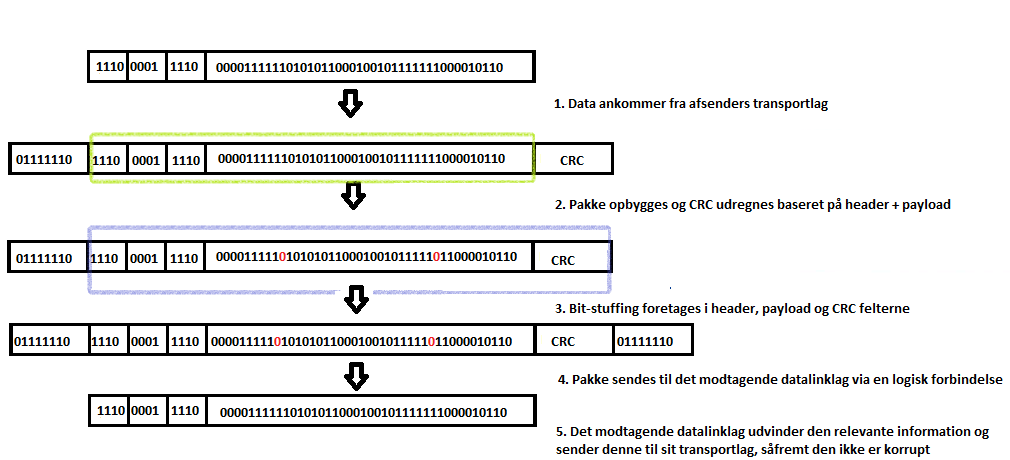
\includegraphics[scale=0.6]{Billeder/DataLinkExample.PNG}
\caption{Eksempel på transmission af en pakke på datalinklaget}
\label{fig:DataLinkExample}
\end{figure}